% Options for packages loaded elsewhere
\PassOptionsToPackage{unicode}{hyperref}
\PassOptionsToPackage{hyphens}{url}
\PassOptionsToPackage{dvipsnames,svgnames,x11names}{xcolor}
%
\documentclass[
  twocolumn,
  landscape]{report}

\usepackage{amsmath,amssymb}
\usepackage{iftex}
\ifPDFTeX
  \usepackage[T1]{fontenc}
  \usepackage[utf8]{inputenc}
  \usepackage{textcomp} % provide euro and other symbols
\else % if luatex or xetex
  \usepackage{unicode-math}
  \defaultfontfeatures{Scale=MatchLowercase}
  \defaultfontfeatures[\rmfamily]{Ligatures=TeX,Scale=1}
\fi
\usepackage{lmodern}
\ifPDFTeX\else  
    % xetex/luatex font selection
\fi
% Use upquote if available, for straight quotes in verbatim environments
\IfFileExists{upquote.sty}{\usepackage{upquote}}{}
\IfFileExists{microtype.sty}{% use microtype if available
  \usepackage[]{microtype}
  \UseMicrotypeSet[protrusion]{basicmath} % disable protrusion for tt fonts
}{}
\makeatletter
\@ifundefined{KOMAClassName}{% if non-KOMA class
  \IfFileExists{parskip.sty}{%
    \usepackage{parskip}
  }{% else
    \setlength{\parindent}{0pt}
    \setlength{\parskip}{6pt plus 2pt minus 1pt}}
}{% if KOMA class
  \KOMAoptions{parskip=half}}
\makeatother
\usepackage{xcolor}
\usepackage[inner=3cm,outer=4cm,top=3cm,bottom=4cm,headsep=22pt,headheight=11pt,footskip=33pt,ignorehead,ignorefoot,heightrounded]{geometry}
\setlength{\emergencystretch}{3em} % prevent overfull lines
\setcounter{secnumdepth}{-\maxdimen} % remove section numbering
% Make \paragraph and \subparagraph free-standing
\makeatletter
\ifx\paragraph\undefined\else
  \let\oldparagraph\paragraph
  \renewcommand{\paragraph}{
    \@ifstar
      \xxxParagraphStar
      \xxxParagraphNoStar
  }
  \newcommand{\xxxParagraphStar}[1]{\oldparagraph*{#1}\mbox{}}
  \newcommand{\xxxParagraphNoStar}[1]{\oldparagraph{#1}\mbox{}}
\fi
\ifx\subparagraph\undefined\else
  \let\oldsubparagraph\subparagraph
  \renewcommand{\subparagraph}{
    \@ifstar
      \xxxSubParagraphStar
      \xxxSubParagraphNoStar
  }
  \newcommand{\xxxSubParagraphStar}[1]{\oldsubparagraph*{#1}\mbox{}}
  \newcommand{\xxxSubParagraphNoStar}[1]{\oldsubparagraph{#1}\mbox{}}
\fi
\makeatother


\providecommand{\tightlist}{%
  \setlength{\itemsep}{0pt}\setlength{\parskip}{0pt}}\usepackage{longtable,booktabs,array}
\usepackage{calc} % for calculating minipage widths
% Correct order of tables after \paragraph or \subparagraph
\usepackage{etoolbox}
\makeatletter
\patchcmd\longtable{\par}{\if@noskipsec\mbox{}\fi\par}{}{}
\makeatother
% Allow footnotes in longtable head/foot
\IfFileExists{footnotehyper.sty}{\usepackage{footnotehyper}}{\usepackage{footnote}}
\makesavenoteenv{longtable}
\usepackage{graphicx}
\makeatletter
\def\maxwidth{\ifdim\Gin@nat@width>\linewidth\linewidth\else\Gin@nat@width\fi}
\def\maxheight{\ifdim\Gin@nat@height>\textheight\textheight\else\Gin@nat@height\fi}
\makeatother
% Scale images if necessary, so that they will not overflow the page
% margins by default, and it is still possible to overwrite the defaults
% using explicit options in \includegraphics[width, height, ...]{}
\setkeys{Gin}{width=\maxwidth,height=\maxheight,keepaspectratio}
% Set default figure placement to htbp
\makeatletter
\def\fps@figure{htbp}
\makeatother
% definitions for citeproc citations
\NewDocumentCommand\citeproctext{}{}
\NewDocumentCommand\citeproc{mm}{%
  \begingroup\def\citeproctext{#2}\cite{#1}\endgroup}
\makeatletter
 % allow citations to break across lines
 \let\@cite@ofmt\@firstofone
 % avoid brackets around text for \cite:
 \def\@biblabel#1{}
 \def\@cite#1#2{{#1\if@tempswa , #2\fi}}
\makeatother
\newlength{\cslhangindent}
\setlength{\cslhangindent}{1.5em}
\newlength{\csllabelwidth}
\setlength{\csllabelwidth}{3em}
\newenvironment{CSLReferences}[2] % #1 hanging-indent, #2 entry-spacing
 {\begin{list}{}{%
  \setlength{\itemindent}{0pt}
  \setlength{\leftmargin}{0pt}
  \setlength{\parsep}{0pt}
  % turn on hanging indent if param 1 is 1
  \ifodd #1
   \setlength{\leftmargin}{\cslhangindent}
   \setlength{\itemindent}{-1\cslhangindent}
  \fi
  % set entry spacing
  \setlength{\itemsep}{#2\baselineskip}}}
 {\end{list}}
\usepackage{calc}
\newcommand{\CSLBlock}[1]{\hfill\break\parbox[t]{\linewidth}{\strut\ignorespaces#1\strut}}
\newcommand{\CSLLeftMargin}[1]{\parbox[t]{\csllabelwidth}{\strut#1\strut}}
\newcommand{\CSLRightInline}[1]{\parbox[t]{\linewidth - \csllabelwidth}{\strut#1\strut}}
\newcommand{\CSLIndent}[1]{\hspace{\cslhangindent}#1}

\makeatletter
\@ifpackageloaded{caption}{}{\usepackage{caption}}
\AtBeginDocument{%
\ifdefined\contentsname
  \renewcommand*\contentsname{Table of contents}
\else
  \newcommand\contentsname{Table of contents}
\fi
\ifdefined\listfigurename
  \renewcommand*\listfigurename{List of Figures}
\else
  \newcommand\listfigurename{List of Figures}
\fi
\ifdefined\listtablename
  \renewcommand*\listtablename{List of Tables}
\else
  \newcommand\listtablename{List of Tables}
\fi
\ifdefined\figurename
  \renewcommand*\figurename{Figure}
\else
  \newcommand\figurename{Figure}
\fi
\ifdefined\tablename
  \renewcommand*\tablename{Table}
\else
  \newcommand\tablename{Table}
\fi
}
\@ifpackageloaded{float}{}{\usepackage{float}}
\floatstyle{ruled}
\@ifundefined{c@chapter}{\newfloat{codelisting}{h}{lop}}{\newfloat{codelisting}{h}{lop}[chapter]}
\floatname{codelisting}{Listing}
\newcommand*\listoflistings{\listof{codelisting}{List of Listings}}
\makeatother
\makeatletter
\makeatother
\makeatletter
\@ifpackageloaded{caption}{}{\usepackage{caption}}
\@ifpackageloaded{subcaption}{}{\usepackage{subcaption}}
\makeatother
<script async src="https://pagead2.googlesyndication.com/pagead/js/adsbygoogle.js?client=ca-pub-1440105407870599" crossorigin="anonymous"></script>

\ifLuaTeX
  \usepackage{selnolig}  % disable illegal ligatures
\fi
\usepackage{bookmark}

\IfFileExists{xurl.sty}{\usepackage{xurl}}{} % add URL line breaks if available
\urlstyle{same} % disable monospaced font for URLs
\hypersetup{
  pdftitle={Chương 2: Phương pháp chiết xuất thường quy},
  pdfauthor={TS. Hoàng Lê Sơn},
  colorlinks=true,
  linkcolor={blue},
  filecolor={Maroon},
  citecolor={Blue},
  urlcolor={Blue},
  pdfcreator={LaTeX via pandoc}}


\title{Chương 2: Phương pháp chiết xuất thường quy}
\author{TS. Hoàng Lê Sơn}
\date{}

\begin{document}
\maketitle

\renewcommand*\contentsname{Table of contents}
{
\hypersetup{linkcolor=}
\setcounter{tocdepth}{2}
\tableofcontents
}
\listoffigures
\listoftables

\section{Tóm tắt}\label{tuxf3m-tux1eaft}

Cao chiết từ thực vật có thể được chiết xuất bằng nhiều phương pháp khác
nhau. Theo cách phân loại hiện tại, các phương pháp này chia thành hai
nhóm gồm các phương pháp thường quy và các phương pháp mới.

Chương này đề cập tới các phương pháp thường quy trong chiết xuất gồm
chiết Soxhlet, chiết ngâm, cất kéo hơi nước. Các phương pháp này sử dụng
dung môi hữu cơ hoặc nước tại áp suất khí quyển.

Dung môi được lựa chọn hướng tới thu được nhóm hoạt chất mong muốn cao
nhất và ít tạp chất. Nguyên tắc chung là dung môi phân cực có thể chiết
được nhóm hợp chất phân cực, trong khi dung môi không phân cực có thể
chọn được nhóm không phân cực. Tuy nhiên, trong thực tế phức tạp hơn do
đa dạng thành phần trong dược liệu với tương tác giữa nhiều yếu tố khác
nhau.

Dung môi trong phương pháp chiết Soxhlet có thể là nước hoặc dung môi
hữu cơ, trong khi cất kéo hơi nước chỉ dùng nước làm dung môi. Chương
này sẽ cung cấp khái niệm cũng như ưu nhược điểm từng phương pháp vừa đề
cập.

\begin{figure}

\centering{

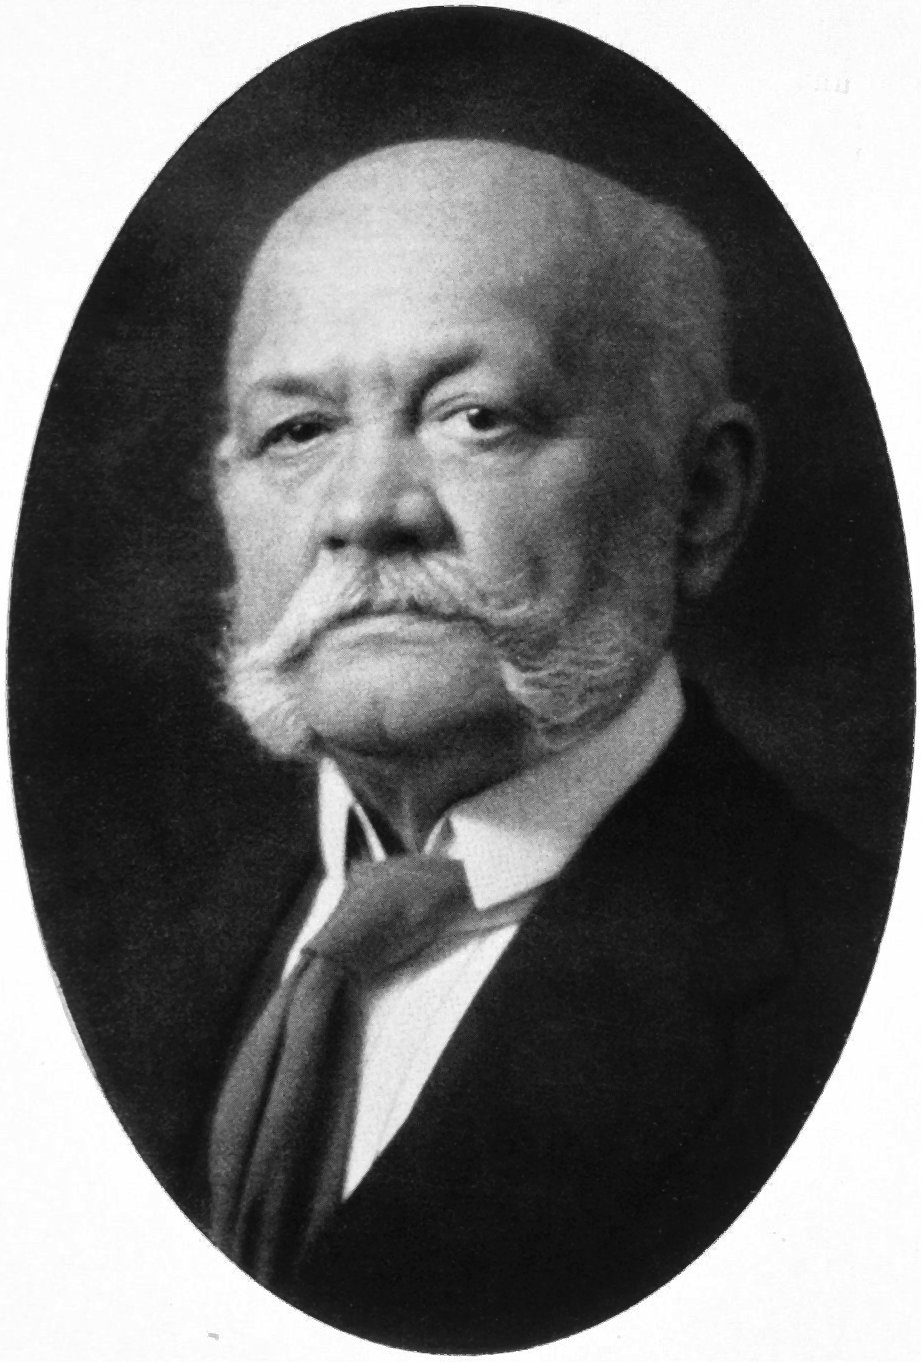
\includegraphics[width=1\textwidth,height=\textheight]{../graphics/Franz_von_Soxhlet.jpg}

}

\caption{\label{fig-Franz}Franz Ritter von Soxhlet (1848 -- 1926) là
người đã phát minh ra thiết bị chiết Soxhlet.}

\end{figure}%

\section{2.1 Chiết Soxhlet và một số thiết bị được cải
tiến}\label{chiux1ebft-soxhlet-vuxe0-mux1ed9t-sux1ed1-thiux1ebft-bux1ecb-ux111ux1b0ux1ee3c-cux1ea3i-tiux1ebfn}

\subsection{2.1.1. Khái quát về chiết
Shoxlet}\label{khuxe1i-quuxe1t-vux1ec1-chiux1ebft-shoxlet}

Chiết xuất bằng Soxhlet là một kỹ thuật thường quy được sử dụng phổ biến
nhất để chiết xuất các hợp chất từ thực vật. Đây là quá trình chiết
lỏng-rắn. Quy trình này dựa trên sự qua trình trao đổi các nhóm chất mục
tiêu từ mẫu chất rắn sang pha lỏng với dung môi lựa chọn phù hợp. Quá
trình này yêu cầu dung môi (pha lỏng) tiếp xúc nhiều nhất với dược liệu
(pha rắn).\textsuperscript{1} Ban đầu, hệ thống chiết bằng Shoxlet được
sử dụng để chiết xuất các lipid nhưng ngày nay được sử dụng với hầu hết
các nhóm chất trong thực vật và từ các bộ phận khác nhau của cây
cỏ.\textsuperscript{2} Một số cái tiến của thiết bị này được phát triển
nhưng nhìn chung mô hình chung vẫn được giữa nguyên. Hiệu quả của phương
pháp chiết bằng Shoxlet phụ thuộc vào khả năng hòa tan của hoạt chất
đích trong dung môi sử dụng với kỳ vọng các tạp chất sẽ không hòa
tan.\textsuperscript{3}

\textbf{Mô tả thiết bị và quá trình chiết:}

\emph{Thuật ngữ tiếng Anh:} Soxhlet Extraction
(Figure~\ref{fig-sohxlet})

\emph{Lịch sử:} Soxhlet là thiết bị do nhà hóa thực vật và phát minh
người Đức phát minh ra vào năm 1879
(Figure~\ref{fig-Franz}).\textsuperscript{4}. Thuật ngữ nhầm lẫn có thể
nhầm lẫn là \emph{Soxtec extraction}. Đây là thiết bị cải tiến từ
Soxhlet được phát triển khoảng thập niên 1970 sau đó thương mại hóa vào
năm 1982. Soxtec là một quy trình hai bước, bao gồm bước đun sôi và bước
rửa, giúp giảm đáng kể tổng thời gian chiết xuất.
(Figure~\ref{fig-soxtec}) Thiết bị đã được sử dụng trong một số ứng dụng
để chiết xuất các chất organochlorine từ các mẫu rắn.

Hệ thống chiết xuất Shoxlet gồm một hệ thống đỡ, một bình chưng cất, xi
phông hình chữ U ngược (tiếng Hy Lạp viết là syphon ) và sinh hàn.
(Figure~\ref{fig-sohxlet}) Hoạt động của thiết bị khá đơn giản, một
lượng mẫu được gói vào trong giấy lọc sau đó đặt ở bình chiết trong khi
đó dung môi được đổ vào bình hứng. Quá trình gia nhiệt bắt đầu, dung môi
sẽ bốc hơi khi đạt nhiệt độ tại bình hứng sẽ ngưng tụ tại bình chiết do
phía trên có sinh hàn. Các hoạt chất trong mẫu sẽ hòa tan vào dung môi
tại bình chiết và khi dung môi tại bình chiết đầy sẽ rút xuống bình hứng
thông qua syphon. Quá trình dung môi từ bình hứng bốc hơi và ngưng tụ
tại bình chiết diễn ra liên tục. Hệ quả là nồng độ của hoạt chất trong
bình chiết tại thời điểm ban đầu sẽ cao hơn nồng độ hoạt chất tại thời
điểm sau và ngược lại khi xem xét nồng độ của hoạt chất trong bình hứng.
Quá trình chiết xuất sẽ dừng lại khi các chất mục tiêu đã chiết kiệt
khỏi mẫu. Dung dịch mẫu cuối cùng không cần lọc sau khi quá trình chiết
suất kết thúc.\textsuperscript{5,6}

\begin{figure}

\centering{

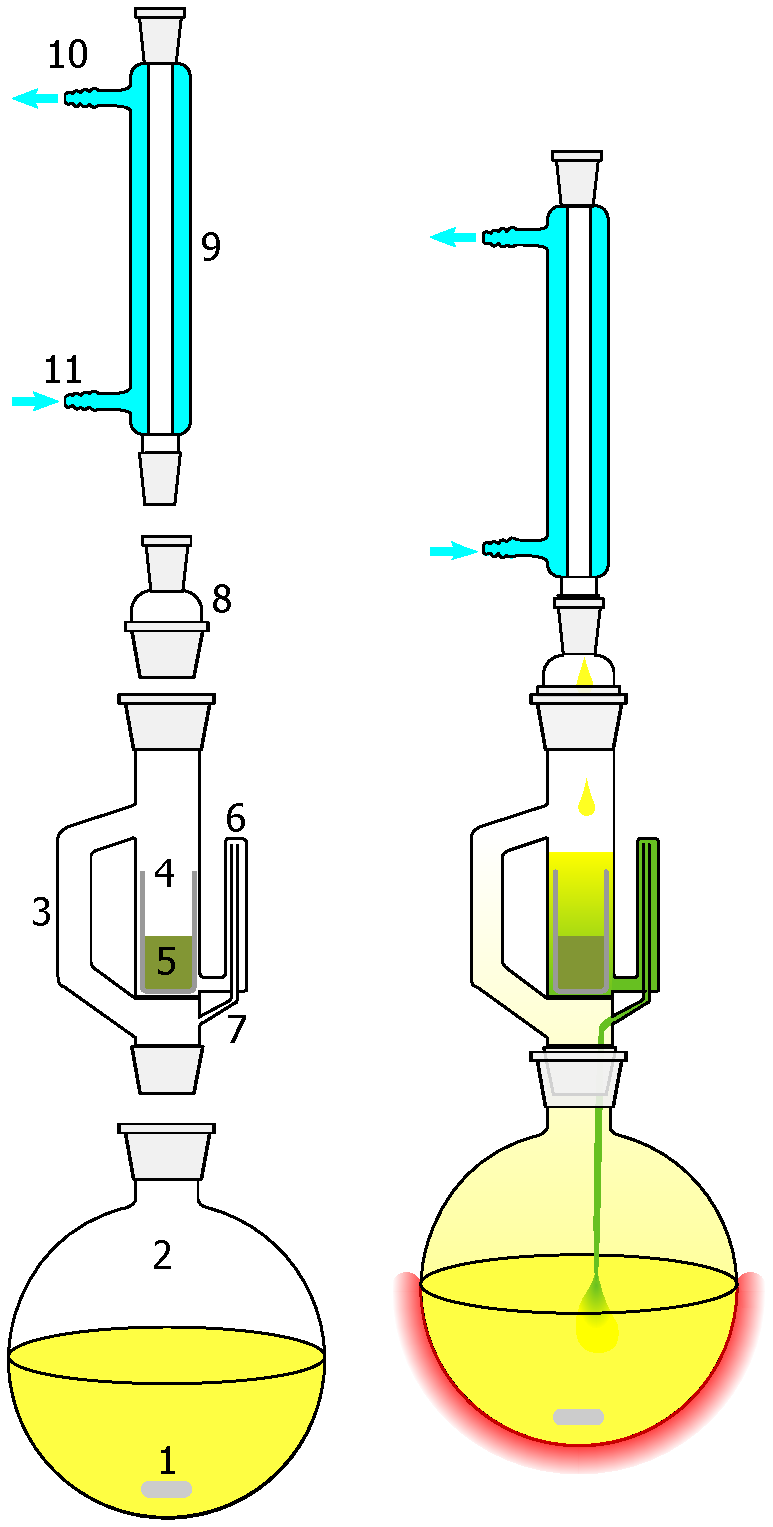
\includegraphics{chapter_2_files/mediabag/../graphics/Soxhlet_extractor.pdf}

}

\caption{\label{fig-sohxlet}Hệ thống chiết Soxhlet là một hệ thống chiết
được cấu tạo gồm hệ thống giá đỡ, một bình chưng cất, syphon và sinh
hàn. Dung môi chiết được lựa chọn phù hợp với chất mục tiêu như n-hexane
dành cho chất kém phân cực như lipid, monoterpen. Nồng độ chất chiết
được trong bình chiết sẽ giảm theo thời gian, trong khi trong bình hứng
sẽ ngược lại.}

\end{figure}%

\begin{figure}

\centering{

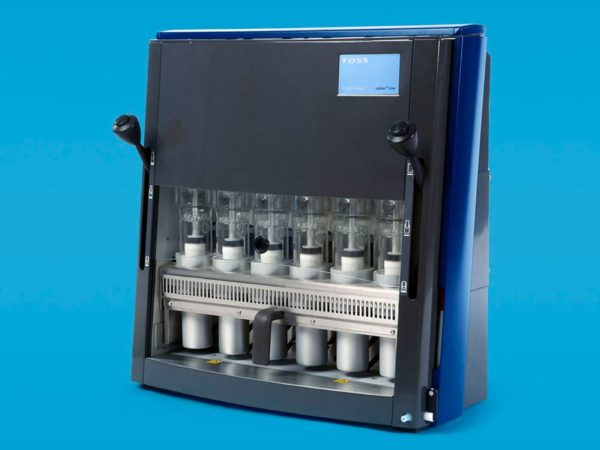
\includegraphics{../graphics/Soxtec.png}

}

\caption{\label{fig-soxtec}Hình ảnh của thiết bị Soxtec của hãng PT Haes
Brothres được phát triển vào những năm 1970 sau đó thương mại vào năm
1982.}

\end{figure}%

\textbf{Ưu điểm và nhược điểm của phương pháp:}

Phương pháp chiết Shoxlet vận hành đơn giản dẫn tới cần ít thời gian đào
tạo nhân công hơn so với các phương pháp khác. Phổ ứng dụng của phương
pháp rộng do phù hợp với nhiều nhóm hợp chất tự nhiên. Nếu so với phương
pháp chiết ngâm, tổng lượng dung môi sử dụng ít hơn trong một mẻ chiết
xuất nguyên nhân là thiết bị hồi lưu dung môi. Thêm nữa, quá trình chiết
suất cũng đồng thời quá trình lọc giúp rút ngắn được thời gian sản xuất
nếu so với các phương pháp chiết khác như phương pháp ngâm. Mặc dù vậy,
quá trình chiết bắt buộc phải có nhiệt để bốc hơi dung môi dẫn tới
phương pháp này chỉ phù hợp với các hoạt chất bền với nhiệt. Dung môi sử
dụng đòi hỏi tinh khiết cao dẫn tới chi phí lớn.\textsuperscript{7} Dĩ
nhiên, phương pháp này cần gia nhiệt trong quá trình chiết xuất vì vậy
tiềm ẩn nguy cơ cháy nổ, kém thân thiện với môi trường nếu so với phương
pháp siêu tới hạn.\textsuperscript{8,9} Thời gian chiết xuất dài nếu so
với một số phương pháp hiện đại hơn như chiết có sự trợ giúp sóng siêu
âm hay chiết xuất có sử dụng áp suất\textsuperscript{10} dẫn tới phương
pháp này không phù hợp để nâng cấp tới quy mô công nghiệp.

\textbf{Một số cải tiến trong hệ thống chiết Shoxlet:}

Do hạn chế nhất định, một số cải tiến đã được đề xuất hướng tới cải
thiện hiệu quả của quá trình chiết xuất.\textsuperscript{11} Subramanian
và cộng sự đã phát triển một hệ thống mới làm giảm thời gian chiết xuất
piperine piperine từ hạt của \emph{Piper nigrum} (hạt tiêu) xuống so với
thiết bị chiết Shoxlet truyền thống khi thêm nhánh dẫn dung môi bốc hơi
từ bình hứng tới bình chiết. (Figure~\ref{fig-sohxletSub}) Shuangqin Ma
và cộng sự năm 2015 cũng đã đề xuất kỹ thuật chiết Shoxlet mới trong đó
thay vì mẫu được gói trong giấy lọc sẽ được hấp thụ trên bề mặt
Silica-gel. Kết quả là có hiệu quả trong chiết xuất flavonoid từ phấn
hoa loài \emph{Brassica campestris} (cây cải dầu).
(Figure~\ref{fig-sohxletShu})\textsuperscript{7}

\begin{figure}

\centering{

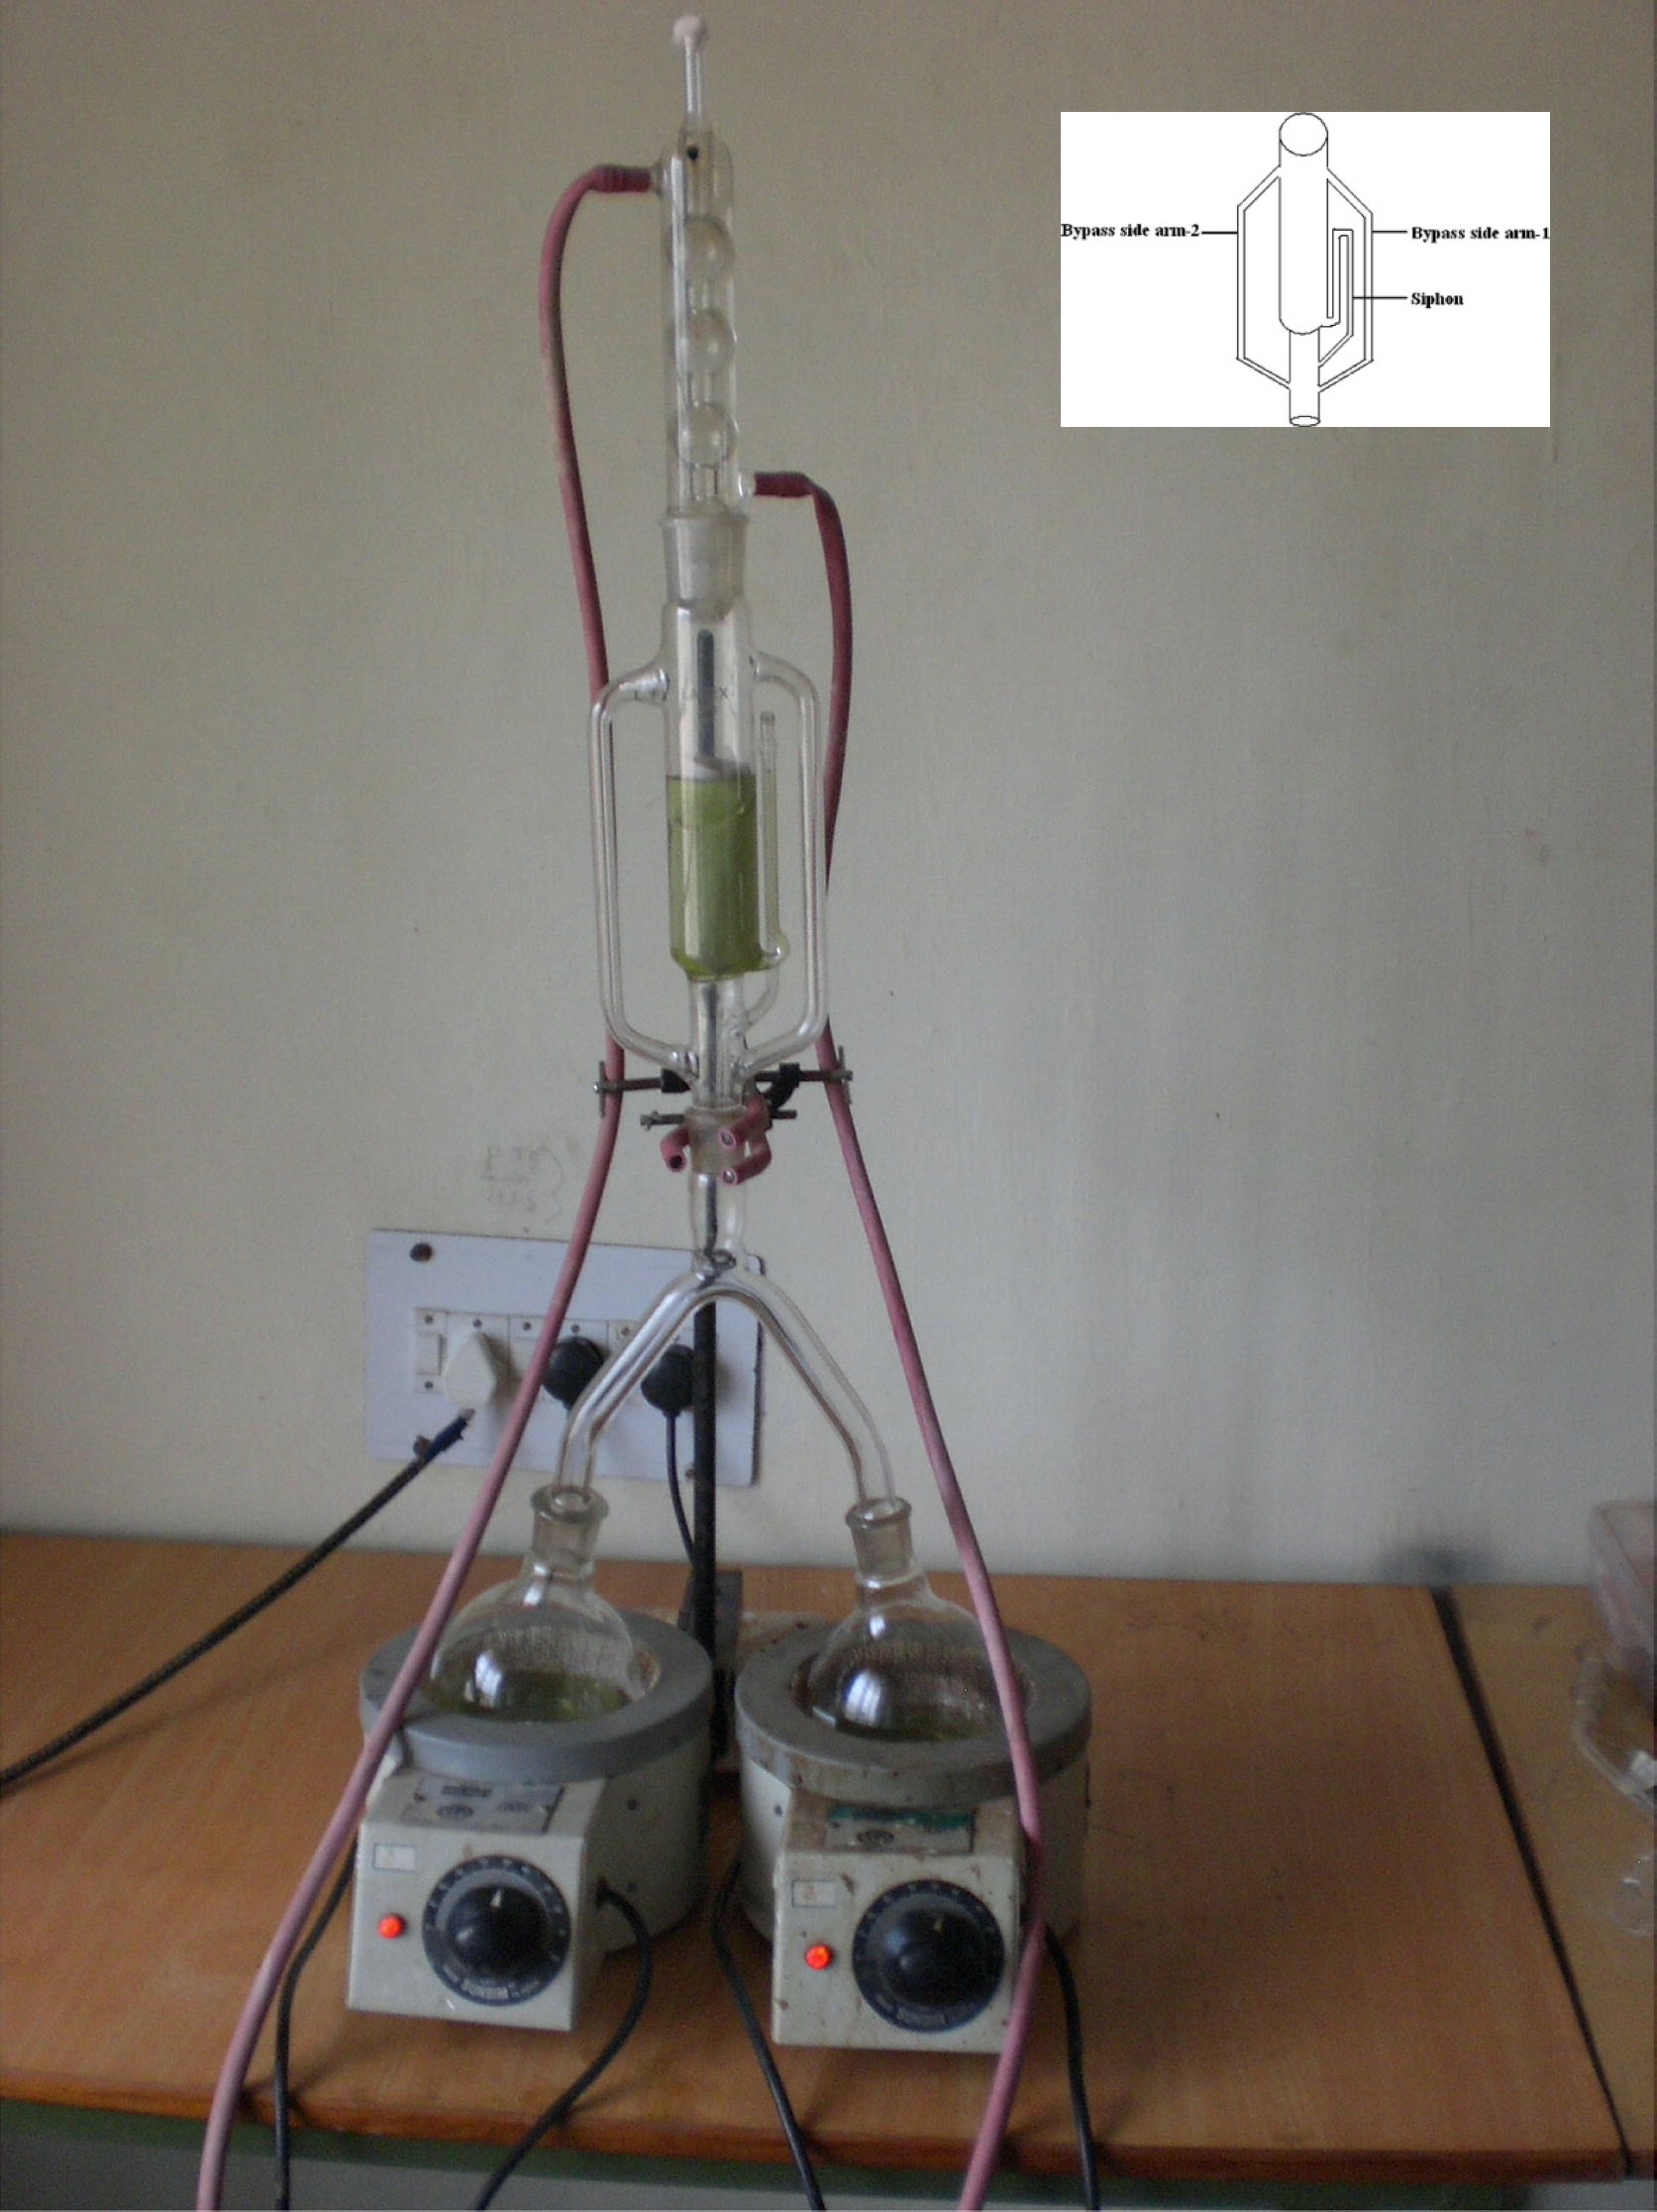
\includegraphics{../graphics/DBSA extraction.jpg}

}

\caption{\label{fig-sohxletSub}Hệ thống cải tiến thiết bị chiết Shoxlet
của Subramanian và cộng sự giúp giảm thời gian chiết piperine từ
\emph{Piper nigrum} khi thêm nhánh dẫn dung môi bốc hơi từ bình hứng tới
bình chiết}

\end{figure}%

\begin{figure}

\centering{

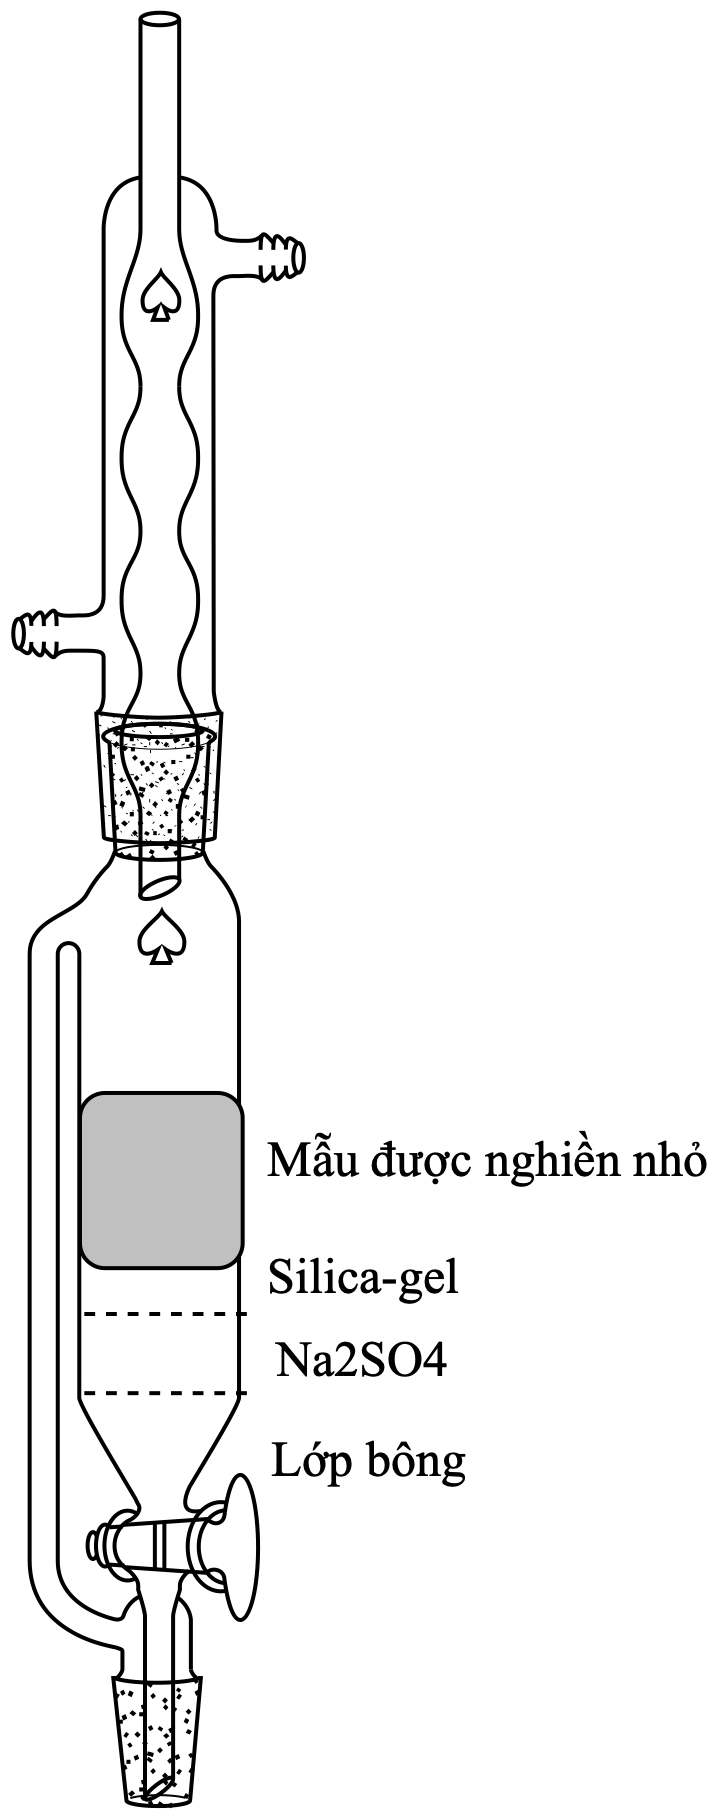
\includegraphics{../graphics/SA-MSPD method.png}

}

\caption{\label{fig-sohxletShu}Shuangqin Ma và cộng sự đã phát triển
phương pháp chuẩn bị mẫu mới trong chiết Shoxlet không cần dùng giấy
lọc. Kết quả giúp tăng hiệu suất chiết flavonoid từ phấn hoa loài
\emph{Brassica campestris} (cây cải dầu)}

\end{figure}%

\subsection{2.1.2 Chiết Soxhlet áp suất
cao}\label{chiux1ebft-soxhlet-uxe1p-suux1ea5t-cao}

\emph{Thuật ngữ tiếng Anh:} High-pressure Soxhlet extraction

Chiết bằng chất lỏng siêu tới hạn kết hợp với chiết Shoxlet được cung
cấp trên thị trường trong phòng thí nghiệm hoặc công nghiệp được thiết
kế trong đó bộ chiết xuất lắp đặt trong bình thép không gỉ.
(Figure~\ref{fig-HighpressureShoxletExtractor}) Mặc dù kết hợp với bộ
chiết siêu tới hạn nhưng điều kiện đạt được sẽ không thu được dung môi
siêu tới hạn. Các dung môi hoặc chất khí sử dụng sẽ có đặc điểm nhiệt độ
sôi thấp ở áp suất và nhiệt độ bình thường, nhưng khi áp suất và nhiệt
độ tăng cao sẽ ở thể lỏng (1000-1500 psi). Với thiết bị này, thơi gian
và lượng dung môi sử dụng có thể giảm đi khoảng một nửa với phương pháp
Soxhlet thuông thường. Thiết bị này này ban đầu được phát triển hướng
tới chiết xuất một hoạt chất trừ sâu như organochlorines và
polychlorinated biphenyls nhưng sau này mở rộng phổ ứng dụng trên các
mẫu có nguồn gốc tự nhiên như cà rốt, khoai tây và dâu ô liu. Dung môi
sử dụng phổ biến nhất là Carbon dioxide với nhiệt độ chiết xuất tại
\(0^oC\). Nhược điểm chính của phương pháp này là quá trình vận hành
phức tạp cộng thêm độ bền của thiết bị cần phải nghĩ tới do hoạt động ở
áp suất cao.\textsuperscript{12,13}

\begin{figure}

\centering{

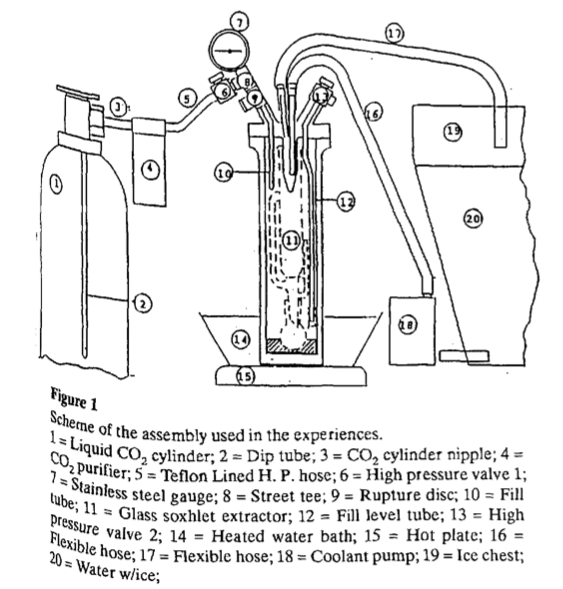
\includegraphics{../graphics/High-pressure Shoxlet Extractor.png}

}

\caption{\label{fig-HighpressureShoxletExtractor}Hệ thống chiết xuất
Shoxlet áp suất cao của Walter G. JenningsRobert H. WohlebNorman W.
Wohlers theo bản quyền số US4265860A của Hoa kỳ. Hệ thống này có thể sử
dụng \(CO_2\) làm dung môi chiết xuất}

\end{figure}%

\subsection{2.1.3 Chiết Soxhlet với trợ giúp bởi siêu
âm}\label{chiux1ebft-soxhlet-vux1edbi-trux1ee3-giuxfap-bux1edfi-siuxeau-uxe2m}

\emph{Thuật ngữ tiếng Anh}: Ultrasound-assisted Soxhlet extraction

Chiết Shoxlet với trợ giúp bởi siêu âm là hệ thống ban đầu được phát
triển để chiết chất béo từ hạt có dầu như hạt hướng dương hay hạt đậu
tương. (\textbf{?@fig-ultraSoxhletExtraction}) Hệ thống này có sử dụng
thiết bị chết Shoxlet truyền thống nhưng bộ phận chiết được đă trong bể
điều nhiệt với đầu dò siều âm. Sự khác biệt giữa thiết bị này với thiết
bị cổ điển là không đáng kể ngoại trừ siêu âm giúp rút ngắn đáng kể chu
kỳ chiết. Sóng siêu âm làm tăng tốc độ giải phóng hoạt chất ra khỏi màng
tế bào. Hệ thống này phù hợp với các nhóm hoạt chất không bền dưới tác
động của oxy.\textsuperscript{14}

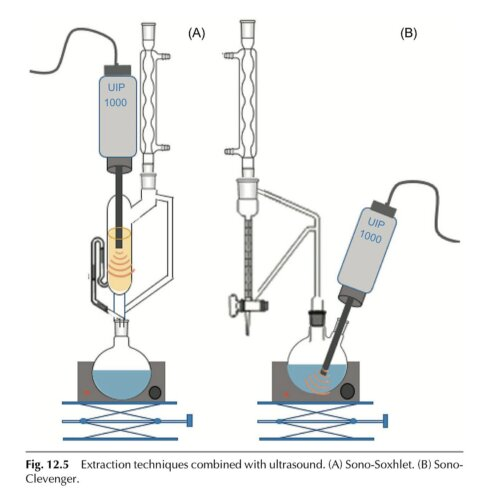
\includegraphics{../graphics/ultrasonic-soxhlet-extraction.png}
\{\#fig-ultraSoxhletExtraction\}

\subsection{2.1.4 Chiết Shoxlet có sự trợ giúp bởi vi
sóng}\label{chiux1ebft-shoxlet-cuxf3-sux1ef1-trux1ee3-giuxfap-bux1edfi-vi-suxf3ng}

\emph{Thuật ngữ tiếng Anh}: Microwave-assisted Soxhlet extraction

Phương pháp chiết Shoxlet có sự trợ giúp bởi vi sóng là kỹ thuật thu
được hiệu quả chiết xuất cao nhất. Sự khác biệt giữa chiết Shoxlet có sự
trợ giúp bởi vi sóng và phương pháp chiết Shoxlet thông thường ở các
điểm sau: (a) áp suất được giữ bình thường khi bình được mở, (b) vi sóng
tập trung tại ngăn chứa dược liệu, (c) như trong chiết Shoxlet thông
thường , giai đoạn chiết xuất được hoàn thành toàn bộ hoặc một phần và
(d) không bao gồm quá trình lọc.
(Figure~\ref{fig-MicrowaveAssistedSoxhletExtraction}) Kết quả là, các
phương pháp này duy trì các ưu điểm của chiết Shoxlet thông thường đồng
thời khắc phục các hạn chế. Đáng chú ý các lợi điểm gồm tốc độ, khả năng
tự động hóa và cũng như khả năng chiết kiệt hoạt chất cần quan
tâm.\textsuperscript{14}

:::

\begin{figure}

\centering{

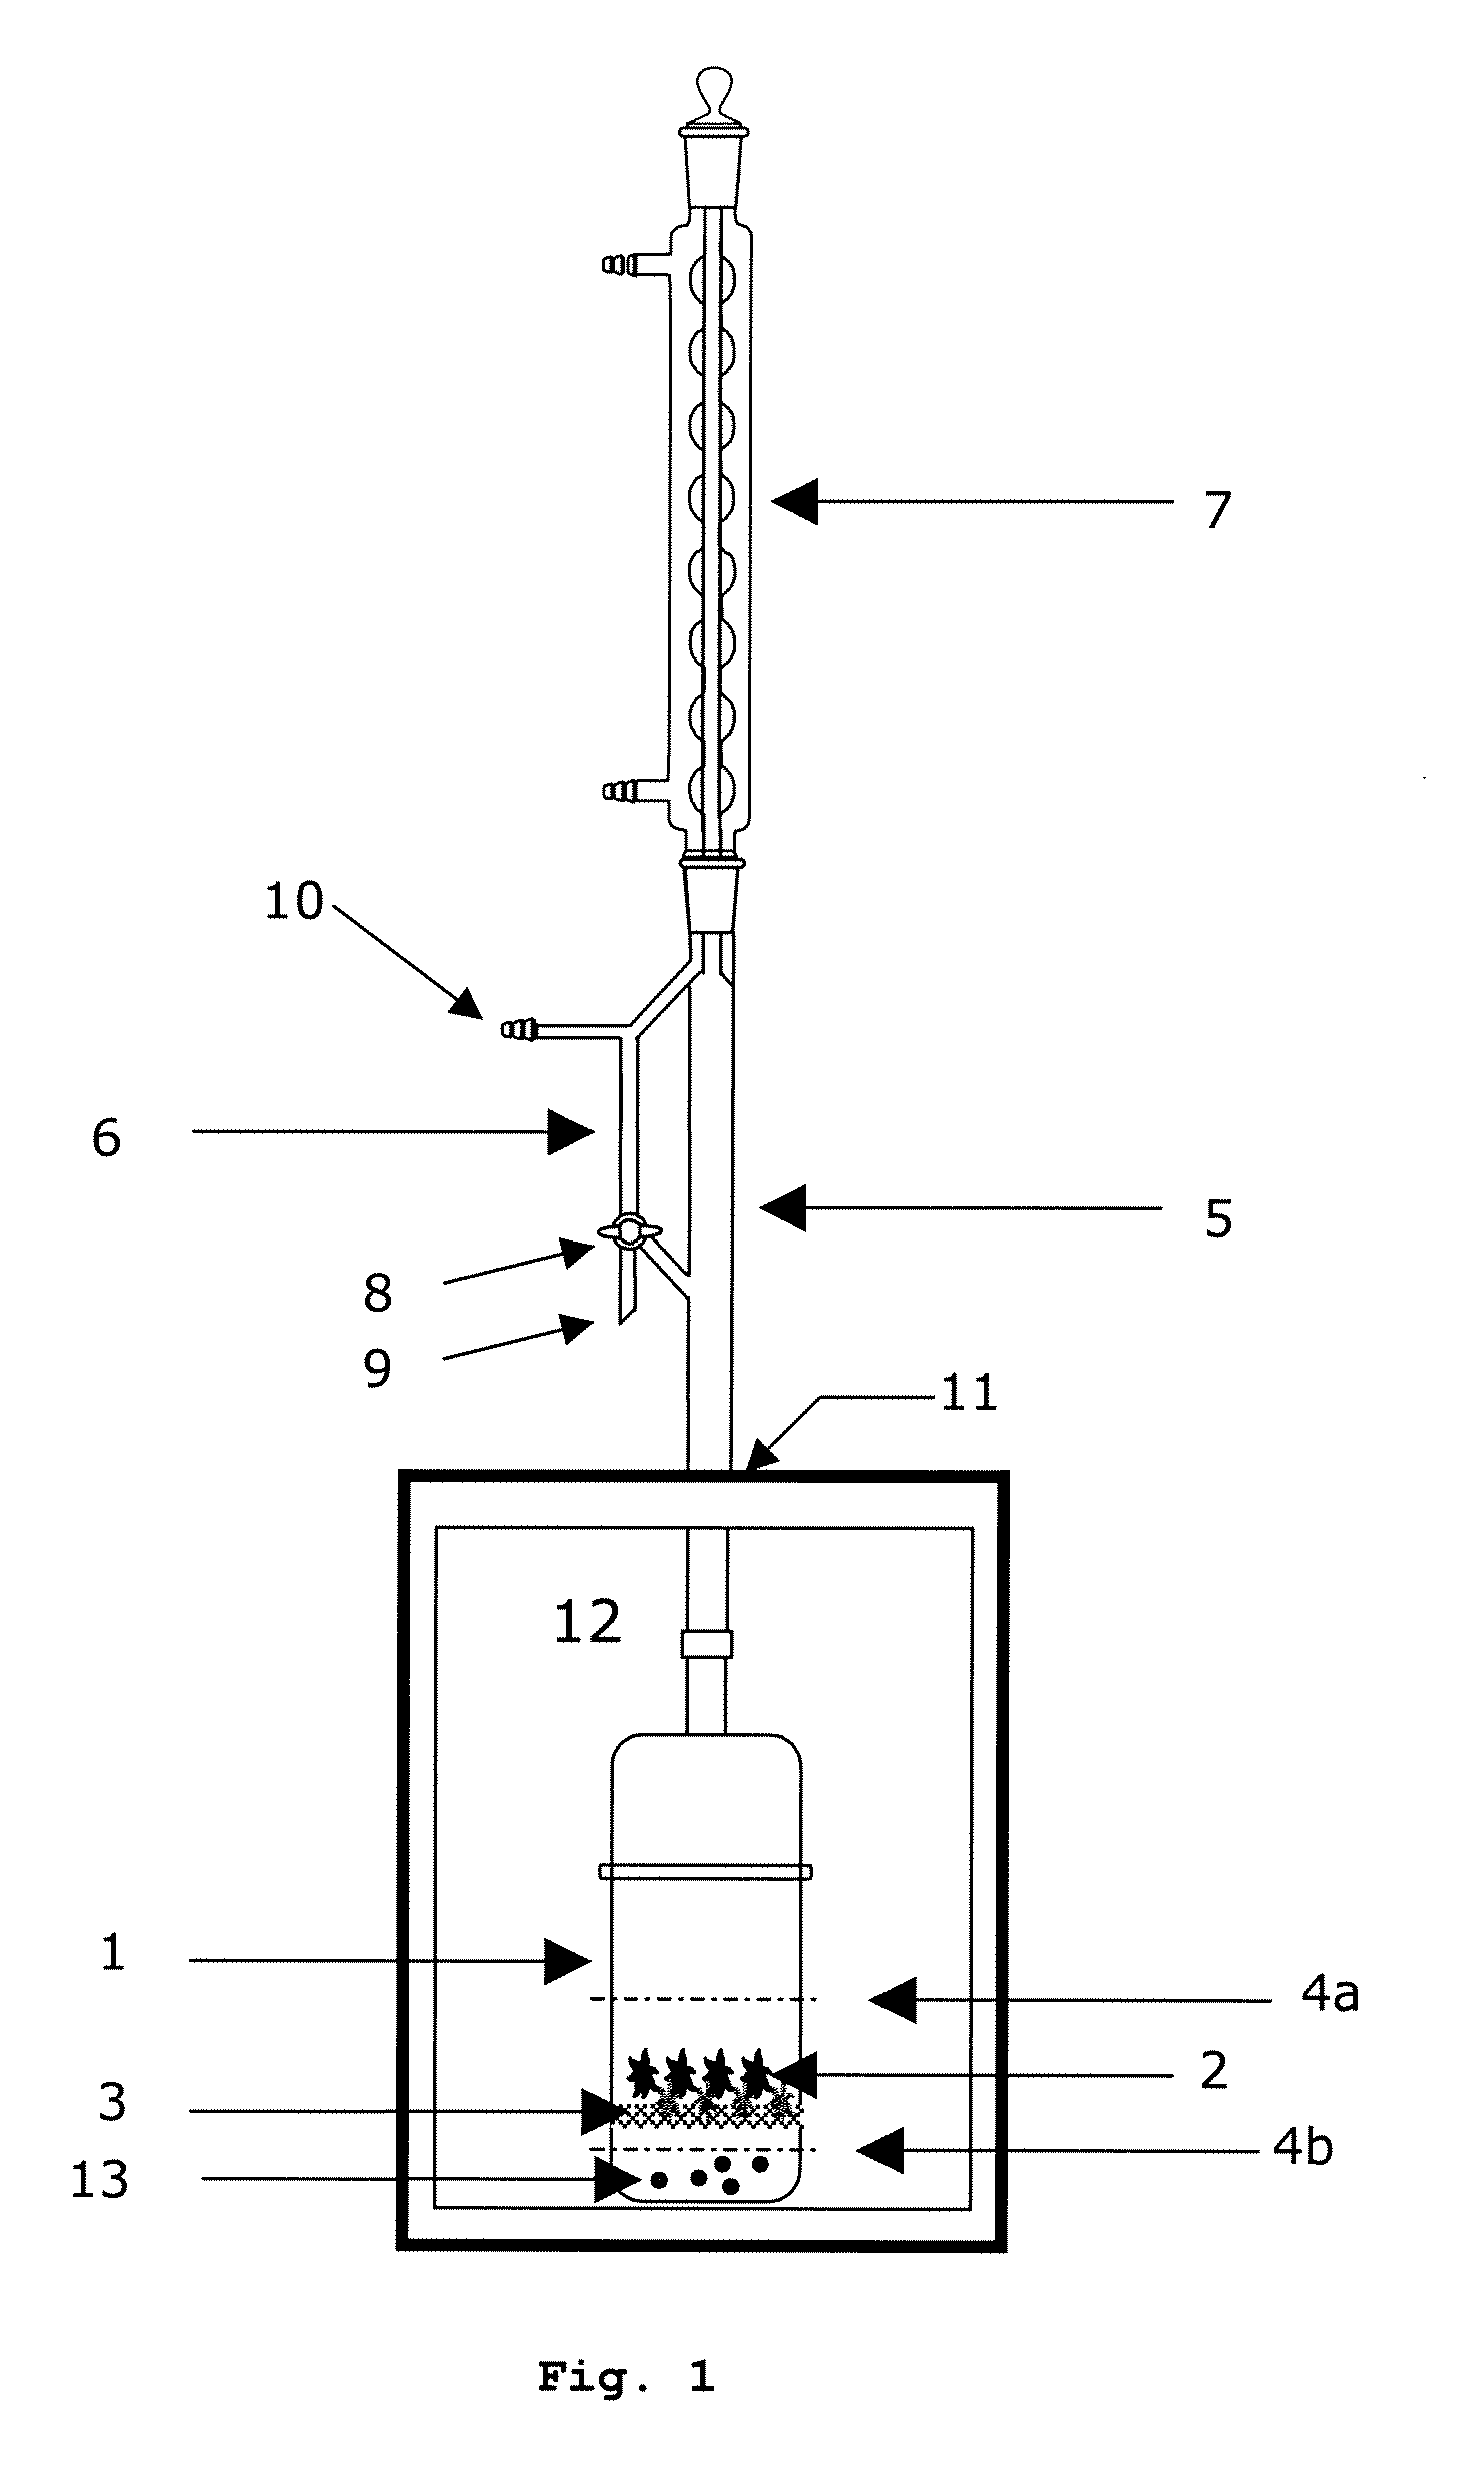
\includegraphics{../graphics/Microwave-assisted Soxhlet extraction.png}

}

\caption{\label{fig-MicrowaveAssistedSoxhletExtraction}Hệ thống chiết
suất Shoxlet có trợ giúp của vi sóng theo bản quyền số EP1955748A1 tại
châu âu. Tác giả bản quyền này là của Farid Universitè d'Avignon et des
Pays de Vaucluse ChematValérie Universitè d'Avignon et des Pays de
Vaucluse TomaoFranco Visinoni}

\end{figure}%

:::

\section{2.2 Chiết ngâm}\label{chiux1ebft-nguxe2m}

\subsection{2.2.1 Khái quát về chiết
ngâm}\label{khuxe1i-quuxe1t-vux1ec1-chiux1ebft-nguxe2m}

\emph{Thuật ngữ tiếng Anh:} Maceration

\emph{Lịch sử:} Chiết ngâm là phương pháp ban đầu để chế rượu thuốc
nhưng sau này được sử dụng để chiết dược liệu. Đây là kỹ thuật phổ biến,
đơn giản và rẻ tiền để chiết xuất.

\textbf{Mô tả thiết bị và quá trình chiết xuất}

Nguyên liệu được nghiền thô cho vật chứa có nắp , sau đó bổ sung thêm
dung môi. Quá trình chiết có yêu cầu khuấy trộn thường xuyên và thời
gian thường diễn tra trong khoảng 3-4 ngày.
(Figure~\ref{fig-LaMaceration}) Nguyên liệu được nghiền thành bột sẽ
tăng diện tích tiếp xúc với dung môi. Ngoài ra, khuấy trộn thường xuyên
cũng tăng khuyếch tan do loại bỏ dung môi đậm đặc khỏi bề mặt mẫu và
chuyển dung môi mới tới bề mặt mẫu. Bước cuối cùng, quá trình lọc là cần
thiết để loại bỏ tạp ra khỏi dung dịch.\textsuperscript{15,16} Điều này
làm tăng tốc độ chiết xuất.\textsuperscript{17}

\begin{figure}

\centering{

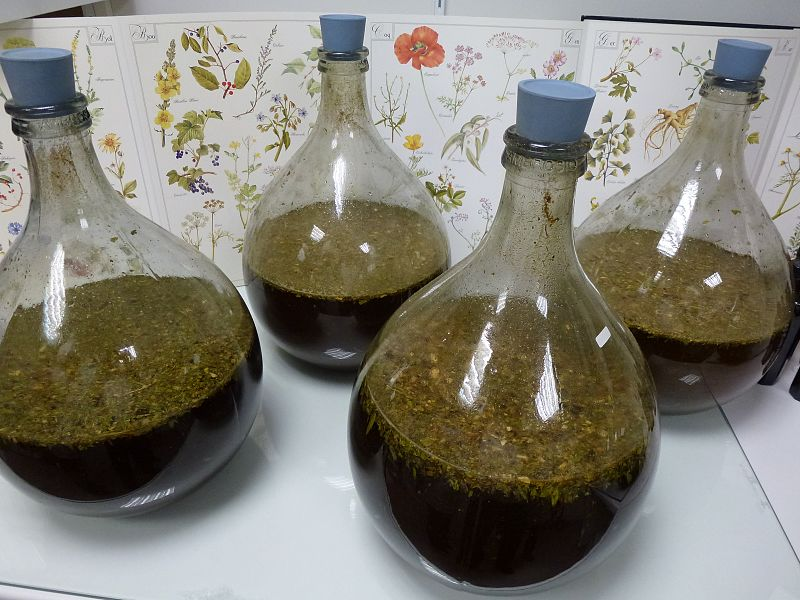
\includegraphics{../graphics/La_maceration.jpg}

}

\caption{\label{fig-LaMaceration}Chiết ngâm là phương pháp chiết dược
liệu đơn giản nhất với thiết bị chỉ cần có nắp đậy.}

\end{figure}%

\textbf{Ưu điểm và giới hạn}

Với hợp chất nhạy cảm với nhiệt, phương pháp này hiệu quả để chiết xuất.
Đây cũng là phương pháp đòi hỏi kỹ thuật đơn giản nhất, rẻ tiền khi
trang thiết bị không cần đầu tư nhiều và phổ biến. Tuy nhiên, phương
pháp này đòi hỏi một lượng lớn dung mỗi dẫn tới nếu dung mỗi hữu cơ sẽ
tạo ra vấn đề về môi trường. Trường hợp quá trình chiết xuất có sử dụng
nhiệt độ sẽ làm giảm thể tích dung môi chiết xuất.

\subsection{2.2.2 Sắc thuốc và pha trà thảo
mộc}\label{sux1eafc-thuux1ed1c-vuxe0-pha-truxe0-thux1ea3o-mux1ed9c}

Đây là phương pháp cơ bản để chiết xuất các thành phần có hoạt tính sinh
học giống phương pháp chiết ngâm. Nguyên liệu được chiết bằng dung môi
nước có gia nhiệt hoặc không. Sự khác biệt duy nhất là thời gian ngắn
hơn và lượng dung môi ít hơn. Tỷ lệ rắn lỏng thường khoảng 1:4 đến 1:16.
Phương pháp này thích hợp để chiết xuất thành phần ở định với nhiệt và
nguyên liệu dạng rắn như cành hay rễ. Thêm nữa, dung môi là nước dẫn tới
hoạt chất thu được thuộc nhóm thân nước. Phương pháp này không đòi hỏi
thiết bị đắt tiền.\textsuperscript{5,10}

\subsection{2.2.3 Chiết lọc có
nhiệt}\label{chiux1ebft-lux1ecdc-cuxf3-nhiux1ec7t}

Phương pháp này có thể hình dung giống như pha cafe phin truyền thống
của Việt nam khi quá trình chiết xuất giống như quá trình ngâm nhưng có
thêm bộ phận lọc. Mẫu được nghiền mịn cho vào thiết bị, sau đó bổ sung
nước sôi ngâm trong 2 giờ. Quá trình này diễn ra với tốc độ vừa phải
(thường 6 giọt trên phút) cho đến khi chiết xuất hoàn toàn. Dịch lọc
cuối cùng sẽ được bay hơi để thu được cao dịch chiết dạng cô
đặc.\textsuperscript{18} Kỹ thuật này sử dụng thiết bị độc đáo được gọi
là máy lọc màu và tuân theo cùng một nguyên tắc cơ bản của quá trình
ngâm. Mẫu đã nghiền mịn được đổ vào máy lọc màu; sau đó, nước sôi được
cho vào và ngâm trong 2 giờ. Quá trình này được thực hiện với tốc độ vừa
phải (sáu giọt mỗi phút) cho đến khi chiết xuất hoàn toàn. Cuối cùng,
quá trình bay hơi được thực hiện để thu được dịch chiết ở dạng cô đặc.

\section{2.3 Phương pháp cất kéo hơi
nước}\label{phux1b0ux1a1ng-phuxe1p-cux1ea5t-kuxe9o-hux1a1i-nux1b0ux1edbc}

\subsection{2.3.1 Khái quát về phương pháp cất kéo hơi
nước}\label{khuxe1i-quuxe1t-vux1ec1-phux1b0ux1a1ng-phuxe1p-cux1ea5t-kuxe9o-hux1a1i-nux1b0ux1edbc}

Cất kéo hơi nước là kỹ thuật chiết xuất thường quy để thu được các tinh
dầu (dầu bay hơi) từ thực vật. Đặc trưng của phương pháp này sẽ sử dụng
dược liệu trước khi khô và không sử dụng dung môi hữu cơ.
(Figure~\ref{fig-Catkeuhoinuoc})\textsuperscript{19} Ba phương pháp cất
kéo hơi nước gồm sử dụng chưng cất nước, nước và hơi nước và cất kéo
bằng nước trực tiếp.\textsuperscript{19,20}

\textbf{Mô tả thiết bị và quá trình chiết xuất}

Với phương pháp cất kéo hơi nước, nguyên liệu được đưa vào một bình sau
đó thêm một lượng nước vừa đủ. Quá trình gia nhiệt bắt đầu làm nước sôi
và hơi nước dẫn vào dược liệu. Sự tiếp xúc hơi nước và dược liệu tăng
tăng giải phóng các hoạt chất từ mô thực vật. Qua trình phân lập tinh
dầu cũng được tiến hành với 3 phương pháp đề cập ở trên. Và cuối cùng là
tách dầu ra khỏi nước dựa trên quá trình làm mát gián tiếp thông qua
sinh hàn. Một cách khác, hỗn hợp ngưng tụ có thể chuyển vào bộ phận
chiết lỏng lỏng để tách lấy tinh dầu. Ví dụ nghiên cứu của Ma và cộng sự
đã đề xuất tách tinh dầu từ cây trầm hương sử dụng dung môi aceton sẽ
cho hiệu suất cao nhất. Cũng trong nghiên cứu này cho thấy không có sự
khác biệt giữa quy mô phòng thí nghiệm và công nghiệp. Phương pháp cất
kéo hơi nước được so sánh với hai phương pháp thường quy gồm chiết
Shoxlet và chiết ngâm được trình bầy trong bảng.

\begin{figure}

\centering{

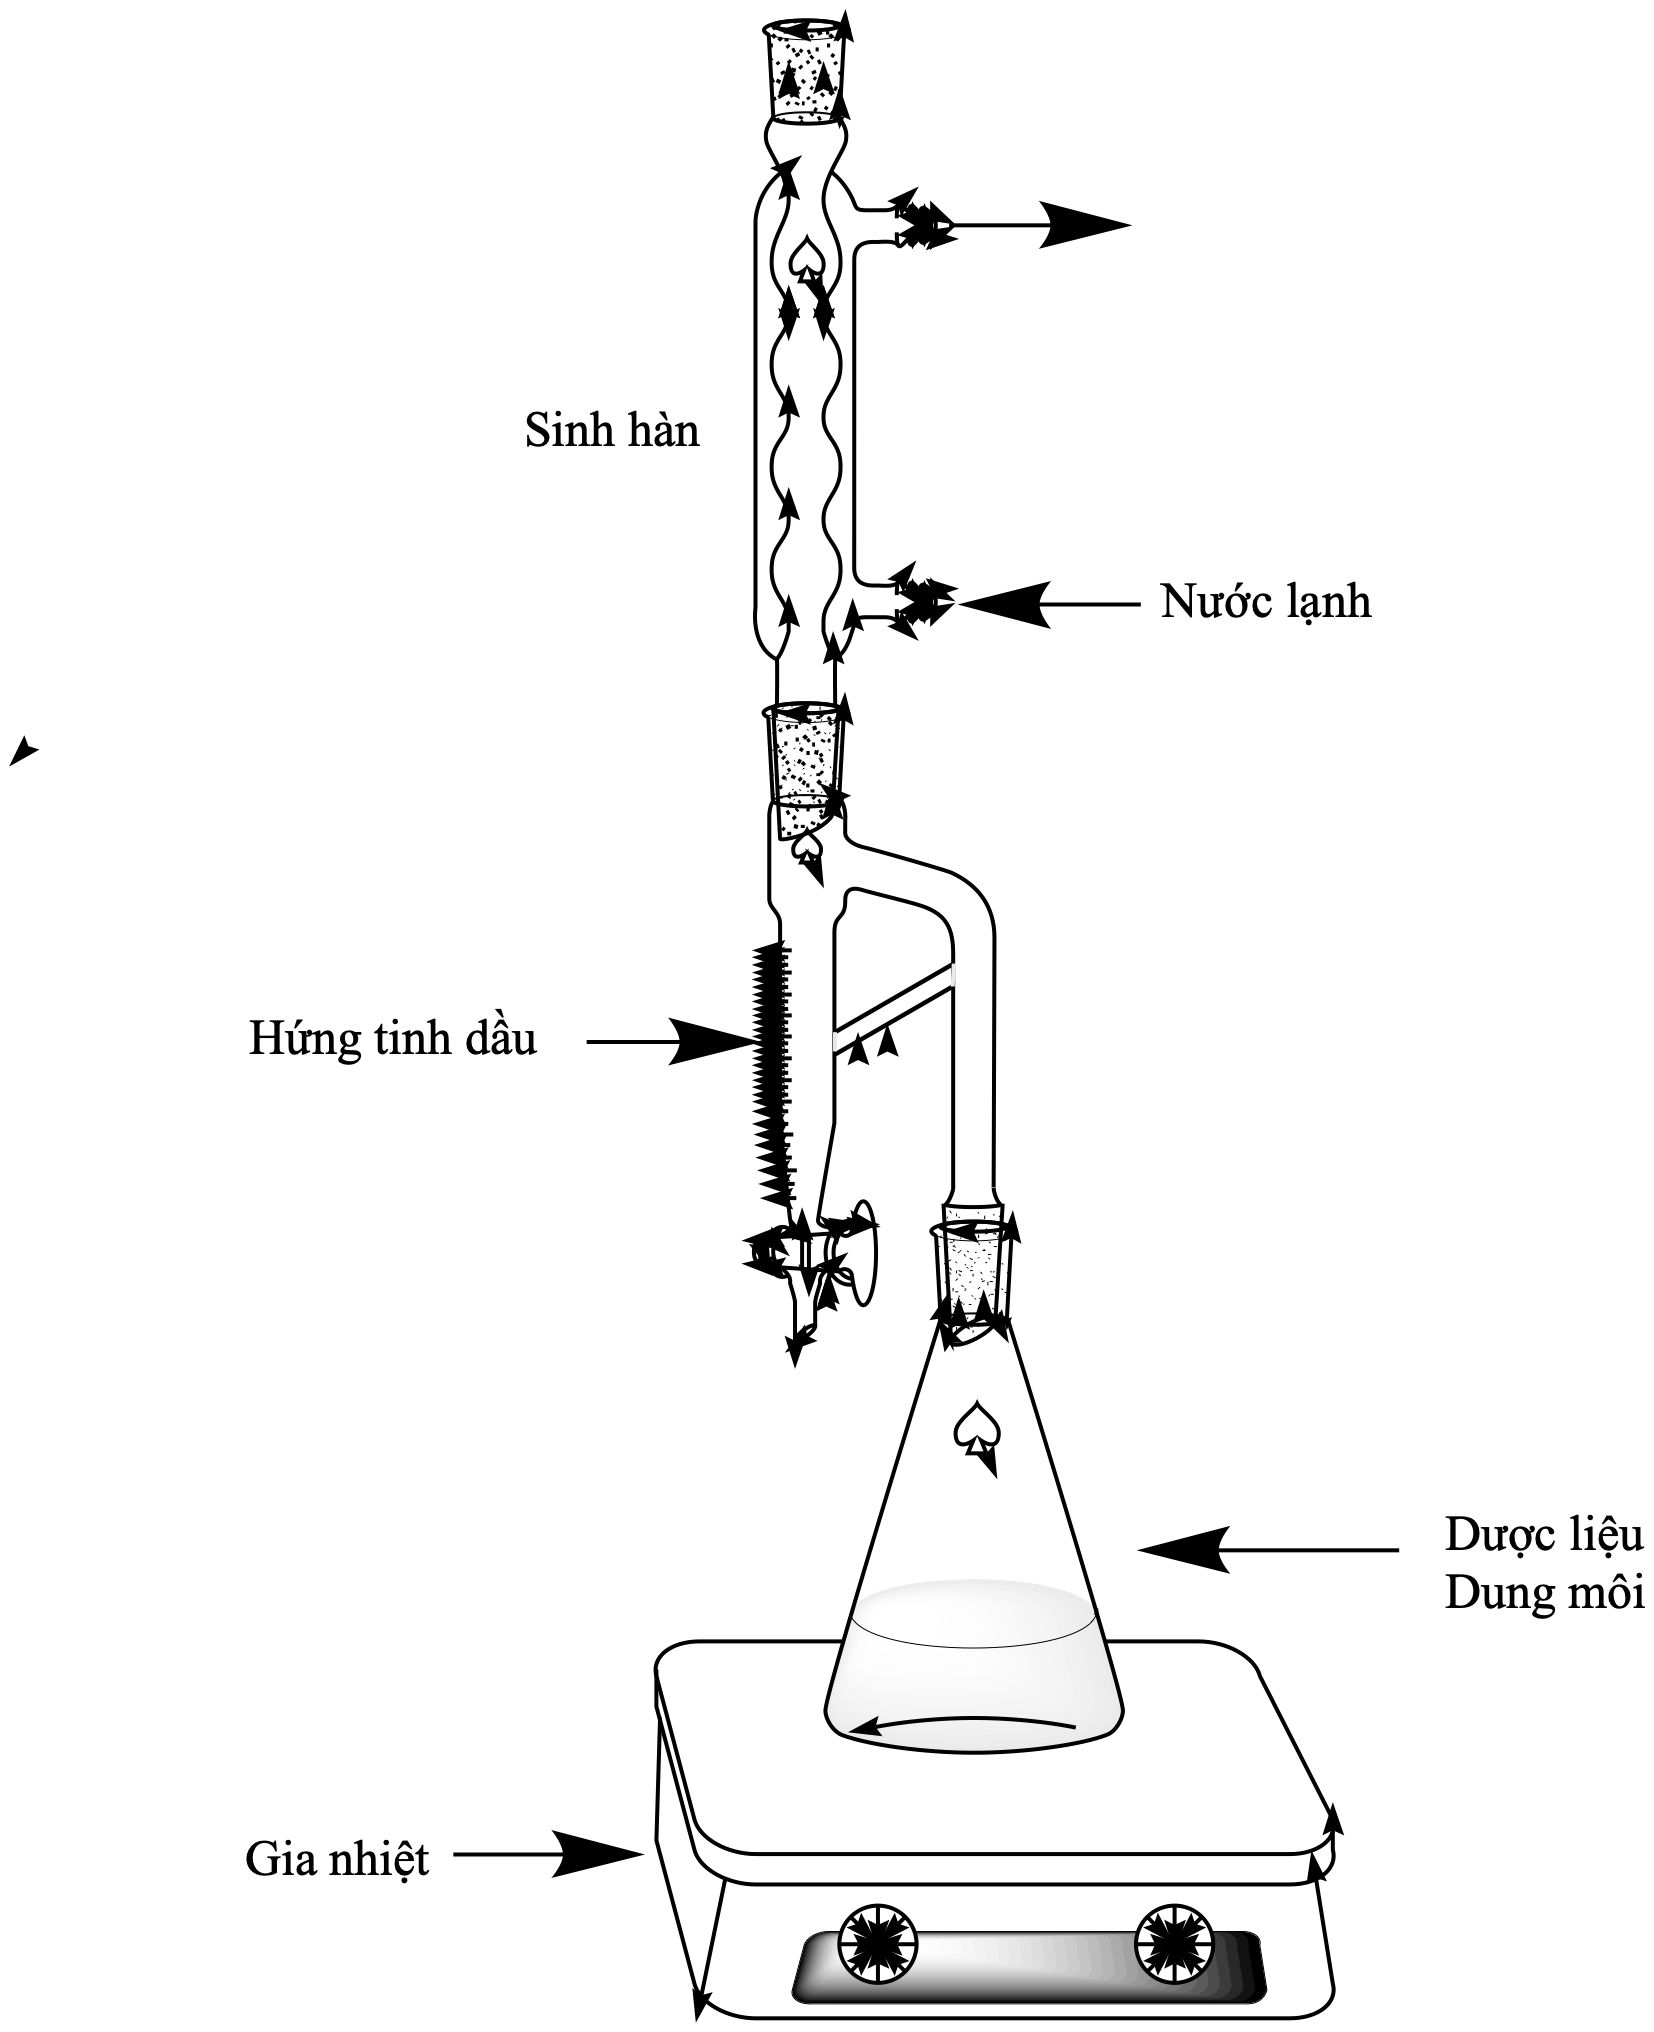
\includegraphics{../graphics/hydrodistillation.png}

}

\caption{\label{fig-Catkeuhoinuoc}Hình ảnh thiết bị cất kéo hơi nước
trong phòng thí nghiệm.}

\end{figure}%

\textbf{Ưu điểm và nhược điểm}

Cất kéo bằng hơi nước được coi là phương pháp thân thiện với môi trường
vì không sử dụng dung môi hữu cơ. Tuy nhiên, hiệu quả kinh tế cũng không
phải tuyệt đối do quá trình cất kéo cần thời gian dài sẽ dẫn tới vấn đề
về nhiên liệu. Ngoài ra, phương pháp không phù hợp với trường hợp hoạt
chất có nhiệt độ sôi cao, nguyên liệu cứng và thân gỗ. Với hợp chất
không bền với nhiệt cũng không áp dụng được phương pháp này.

\subsection{2.3.2 Chưng cất thu tinh
dầu}\label{chux1b0ng-cux1ea5t-thu-tinh-dux1ea7u}

\emph{Thuật ngữ tiếng Anh:} Water distillation
(Figure~\ref{fig-WaterDistillation})

Dược liệu được ngập trong nước, sau đó, đun sôi trong bình tạo ra hơi
nước bốc hơi. Đặc điểm cơ bản của phương pháp này là nước sôi tiếp xúc
trực tiếp với dược liệu. Khi nước nóng lên, cần khuấy ở dược liệu nếu
không dược liệu sẽ tích tụ ở đấy nồi và ảnh hưởng bởi nhiệt. Nếu dược
liệu chứa nhiều chất nhày ví dụ vỏ quế thì phải nghiền thành bột trước
khi chưng cất. Khi nhiệt độ nóng lên, chất nhầy sẽ được chiết ra, tạo độ
nhớt cho dung môi. Đây cũng là một lợi thế của phương pháp. Nếu sử dụng
phương pháp trực tiếp sử dụng hơi nước dẫn vào dược liệu, dược liệu sẽ
tạo ra lớp áo và vón cục ngăn cách dược liệu với hơi nước. Đây chính là
lợi thế của phương pháp này. Tuy nhiên, phương pháp nàu cũng có nhược
điểm là không chiết kiệt được. Thêm nữa, do tiếp xúc trực tiếp với nước
một số thành phần như Aldehyd hay ester của tinh dầu sẽ bị thủy phân.
Phương pháp này được lựa chọn sau cùng khi hai phương pháp sau đây không
phù hợp.

\begin{figure}

\centering{

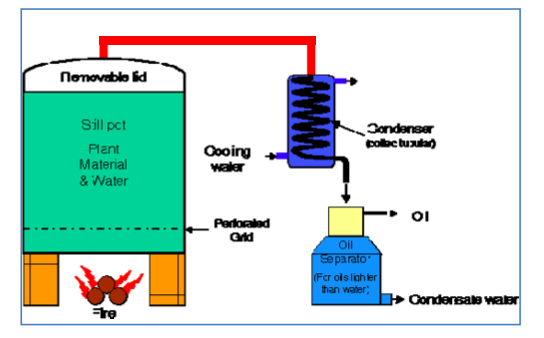
\includegraphics{../graphics/Water distillation.png}

}

\caption{\label{fig-WaterDistillation}Thiết bị chưng cất trực tiếp thu
tinh dầu theo đó dược liệu ngập trong nước và đun sôi để thu tinh dầu.}

\end{figure}%

\subsection{2.3.3 Nước và hơi
nước}\label{nux1b0ux1edbc-vuxe0-hux1a1i-nux1b0ux1edbc}

\emph{Thuật ngữ tiếng Anh:} Water and Steam Distillation
(Figure~\ref{fig-WaterSteamDistillation})

Khác biệt so với phương pháp chưng cất nước là phương pháp dược liệu
không tiếp xúc trực tiếp với nước mà được treo trên dàn đặt ngay phía
trên vùng nước. Sự kết hợp giữa phương pháp chưng cất nước và phương
pháp này trở lên phổ biến tại các cơ sở sản xuất nhỏ lẻ. Tuy nhiên, chất
lượng tinh dầu thu được bằng phương pháp kết hợp này thường không được
đánh giá cao. Để giải quyết, một sự thay đổi nhỏ của phương pháp chưng
cất nước là nguyên liệu sẽ được treo nổi trên bề mặt nước. Cách làm này
làm giảm công suất nhưng chất lượng tinh dầu lại cao hơn. Phương pháp
nước và hơi nước đảm bảo lượng nước sẽ không bị cạn do có thể tái bổ
sung nước theo cách thủ công.

\begin{figure}

\centering{

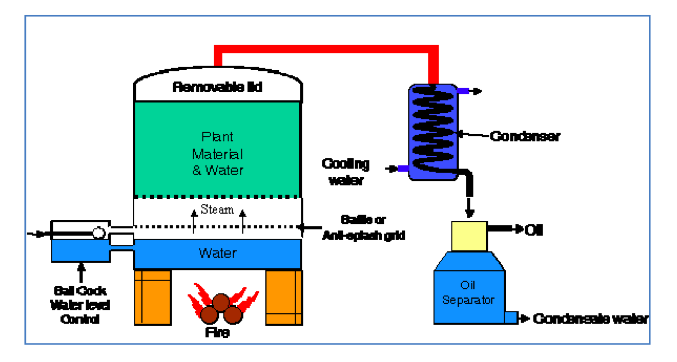
\includegraphics{../graphics/Water and steam distillation.png}

}

\caption{\label{fig-WaterSteamDistillation}Thiết bị chưng cất tinh dầu
trong đó dược liệu không trực tiếp tiếp xúc với nước và dùng hơi nước
bốc hơi để thu tinh dầu.}

\end{figure}%

\subsection{2.3.4 Hơi nước trực
tiếp}\label{hux1a1i-nux1b0ux1edbc-trux1ef1c-tiux1ebfp}

\emph{Thuật ngữ tiếng Anh:} Direct Steam Distillation
(Figure~\ref{fig-DirectSteamDistillation})

Phương pháp này một nồi hơi tạo hơi nước được tách biệt với bộ phận để
nguyên liệu. Nguyên liệu sẽ để trên một giàn lưới sao cho hơi nước có
thể đi qua. Với việc điều chỉnh lượng hơi nước đi qua là một lợi thế của
phương pháp này. Nồi hơi có thể tạo ra nhiệt độ tới \(100^oC\) nhưng
không ảnh hưởng tới dược liệu và hạn chế quá trình thủy phân. Phương
pháp này thường được sử dụng để chiết tinh dầu ở quy mô công nghiệp và
với ngành kinh doanh hương liệu và hương thơm đây chính là thiết bị tiêu
chuẩn. Nhược điểm lớn nhất phương pháp này là vốn đầu tư lớn trong khi
nếu chỉ sản xuất các loại tinh dầu giá trị thấp (như sả và oải hương) có
thể sẽ không thu hồi được vốn bỏ ra trong vòng 10 năm.

\begin{figure}

\centering{

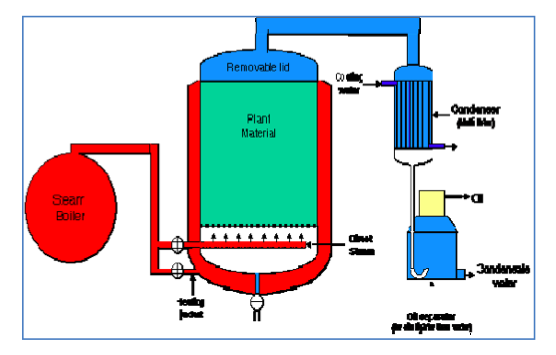
\includegraphics{../graphics/Direct steam distillation.png}

}

\caption{\label{fig-DirectSteamDistillation}Thiết bị chưng cất tinh dầu
trong đó hơi nước được dẫn qua ống để tiếp xúc với dược liệu.}

\end{figure}%

\section{2.4 Giới hạn của phương pháp thường
quy}\label{giux1edbi-hux1ea1n-cux1ee7a-phux1b0ux1a1ng-phuxe1p-thux1b0ux1eddng-quy}

Trong chiết xuất, có nhiều phương pháp chiết xuất và mỗi cách sẽ có một
mục đích nhất định để chiết một nhóm chất nhất định. Cải thiện hiệu suất
chiết có thể thể sử dụng các biện pháp như gia nhiệt hoặc khuấy. Phần
dưới đây đề cập tới từng phương pháp, thông số, ưu điểm và nhược điểm.

\begin{enumerate}
\def\labelenumi{\arabic{enumi}.}
\tightlist
\item
  Chiết Shoxlet
\end{enumerate}

\begin{itemize}
\tightlist
\item
  Thông số: Tỷ lệ chất rắn/dung môi, nhiệt độ, thời gian chiết
\item
  Ưu điểm: Phương pháp đơn giản, nhiệt độ có thể tăng để cải thiện hiệu
  suất.
\item
  Nhược điểm: Hiệu quả trong khai thác thấp, năng lượng sử dụng nhiều và
  tốn thời gian.
\end{itemize}

\begin{enumerate}
\def\labelenumi{\arabic{enumi}.}
\setcounter{enumi}{1}
\tightlist
\item
  Chiết ngâm
\end{enumerate}

\begin{itemize}
\tightlist
\item
  Thông số:Tốc độ dung môi vào, tốc độ rút dung môi, tốc độ hòa tan.
\item
  Ưu điểm: Đầu tư ban đầu thấp, có thể điều chỉnh chọn lọc hoạt chất dựa
  trên dung môi.
\item
  Nhược điểm: Nếu dùng nhiệt để tăng tốc độ sẽ không phù hợp với hoạt
  chất không bền.
\end{itemize}

\begin{enumerate}
\def\labelenumi{\arabic{enumi}.}
\setcounter{enumi}{2}
\tightlist
\item
  Cất kéo hơi nước
\end{enumerate}

\begin{itemize}
\tightlist
\item
  Thông số: Nhiệt độ, thời gian.
\item
  Ưu điểm: Nước tách các hợp chất hoạt tính sinh học khỏi nguyên liệu;
  không sử dụng dung môi hữu cơ.
\item
  Nhược điểm: Nhiệt độ chiết cao có thể làm mất hoạt chất.
\end{itemize}

Khi so sánh với các quy trình khác, chẳng hạn như với chiết ngâm, phương
pháp chiết Shoxhlet sử dụng ít dung môi hơn tuy nhiên nhược điểm phát
sinh khí độc hại và dung môi có khả năng gây cháy. Lựa chọn dung môi có
độ tinh khiết cao có thể làm tăng chi phí sản xuất. So với phương pháp
hiện đại hơn như chiết siêu tới hạn thì phương pháp này lại coi là không
thân thiện với môi trường. Kích thước tiểu phân của mẫu dạng bột mịn
được xem là cách chuẩn bị tốt nhất cho chiết bằng Shoxlet bên cạnh cần
xem xét các yếu tố như nhiệt độ, tỷ lệ rắn/lỏng, tốc độ khuấy và thời
gian. Chiết ngâm trở lên phổ biến với nghiên cứu dược liệu. Phương pháp
này làm mềm dược liệu, hòa tan thành tế bào và giải phóng hoạt chất.
Phương pháp này có ưu điểm như quá trình đơn giản, không sử dụng dung
môi hữu cơ và thời gian chiết nhanh. Nhưng hạn chế có một số nhóm hoạt
chất nhạy cảm với nhiệt. Tương tự với sắc thuốc hay chiết nhỏ giọt.
Phương pháp cất kéo hơi nước có thể có một số nhược điểm như dược liệu
tiếp xúc ở đáy nồi có thể bị cháy, tạo ra mùi khó chịu. Hơn nữa điều
chỉnh nhiệt độ sẽ ảnh hưởng tới tốc độ cất kéo.

\section{2.5 Tổng kết}\label{tux1ed5ng-kux1ebft}

Chiết xuất là bước đầu tiên trong việc phân lập và tinh chế các hợp chất
từ tự nhiện. Do bản chất không hòa tan, các chất chuyển hóa thứ cấp bao
gồm acid phenolic và flavonoid rất khó chiết xuất. Mặc dù, các phương
pháp chiết xuất thường quy cụ thể là chiết Shoxhlet, chiết ngâm, cất kéo
hơi nước là những cách hiệu quả để chiết xuất nhưng có nhiều loại trang
thiết bị khác nhau. Nhưng nhìn chung các phương pháp này có nhược điểm
không phù hợp với chất nhạy cảm với nhiệt, tốn thời gian, tính chọn lọc
kém và có thể gây ô nhiễm. Khi đề cập tới chiết xuất, mục tiêu phải chọn
được phương pháp phù hợp để chiết nhóm có hoạt tính, hiệu quả trong vận
hành, chi phí sản xuất thấp. Do đó, gần đây các cải tiến phương pháp
liên tục được đề xuất song vẫn cần tiếp tục nghiên cứu thêm để giải
quyết nhu cầu thị trường ngày càng tăng.

\section{2.6 Câu hỏi lượng
giá}\label{cuxe2u-hux1ecfi-lux1b0ux1ee3ng-giuxe1}

Câu 1: Mô tả thiết bị chiết Soxhlet Câu 2: Phân tích ưu và nhược điểm
thiết bị chiết Soxhlet. Các cải tiến cho chiết bị chiết Soxhlet đã được
áp dụng Câu 3: Mô tả thiết bị chiết

\phantomsection\label{refs}
\begin{CSLReferences}{0}{0}
\bibitem[\citeproctext]{ref-castro_bacterial_2012}
\CSLLeftMargin{1 }%
\CSLRightInline{\href{https://doi.org/10.1016/j.carbpol.2012.03.045}{C.
Castro, R. Zuluaga, C. Álvarez, J.-L. Putaux, G. Caro, O. J. Rojas, I.
Mondragon and P. Gañán, \emph{Carbohydrate Polymers}, 2012, \textbf{89},
1033--1037}.}

\bibitem[\citeproctext]{ref-yang_selective_2013}
\CSLLeftMargin{2 }%
\CSLRightInline{\href{https://doi.org/10.1016/j.jhazmat.2013.03.026}{F.
Yang, F. Kubota, Y. Baba, N. Kamiya and M. Goto, \emph{Journal of
Hazardous Materials}, 2013, \textbf{254--255}, 79--88}.}

\bibitem[\citeproctext]{ref-punin_crespo_comparison_2006}
\CSLLeftMargin{3 }%
\CSLRightInline{\href{https://doi.org/10.1016/j.ecoenv.2005.04.010}{M.
O. Punín Crespo and M. A. Lage Yusty, \emph{Ecotoxicology and
Environmental Safety}, 2006, \textbf{64}, 400--405}.}

\bibitem[\citeproctext]{ref-jensen_origin_2007}
\CSLLeftMargin{4 }%
\CSLRightInline{\href{https://doi.org/10.1021/ed084p1913}{W. B. Jensen,
\emph{J. Chem. Educ.}, 2007, \textbf{84}, 1913}.}

\bibitem[\citeproctext]{ref-bimakr_comparison_2011}
\CSLLeftMargin{5 }%
\CSLRightInline{\href{https://doi.org/10.1016/j.fbp.2010.03.002}{M.
Bimakr, R. A. Rahman, F. S. Taip, A. Ganjloo, L. M. Salleh, J. Selamat,
A. Hamid and I. S. M. Zaidul, \emph{Food and Bioproducts Processing},
2011, \textbf{89}, 67--72}.}

\bibitem[\citeproctext]{ref-arthur_soxhlet_nodate}
\CSLLeftMargin{6 }%
\CSLRightInline{\href{https://patents.google.com/patent/EP0747103A1/en}{0747103A1,
}.}

\bibitem[\citeproctext]{ref-ma_soxhlet-assisted_2015}
\CSLLeftMargin{7 }%
\CSLRightInline{\href{https://doi.org/10.1016/j.jchromb.2015.09.038}{S.
Ma, X. Tu, J. Dong, P. Long, W. Yang, X. Miao, W. Chen and Z. Wu,
\emph{Journal of Chromatography B}, 2015, \textbf{1005}, 17--22}.}

\bibitem[\citeproctext]{ref-buss_natural_2009}
\CSLLeftMargin{8 }%
\CSLRightInline{A. D. Buss and M. S. Butler, Eds.,
\emph{\href{https://doi.org/10.1039/9781847559890}{Natural product
chemistry for drug discovery}}, Royal Society of Chemistry, Cambridge,
2009.}

\bibitem[\citeproctext]{ref-punin_crespo_comparison_2005}
\CSLLeftMargin{9 }%
\CSLRightInline{\href{https://doi.org/10.1016/j.chemosphere.2004.12.025}{M.
O. Punín Crespo and M. A. Lage Yusty, \emph{Chemosphere}, 2005,
\textbf{59}, 1407--1413}.}

\bibitem[\citeproctext]{ref-nn_review_2015}
\CSLLeftMargin{10 }%
\CSLRightInline{A. NN, \emph{Med Aromat Plants},
DOI:\href{https://doi.org/10.4172/2167-0412.1000196}{10.4172/2167-0412.1000196}.}

\bibitem[\citeproctext]{ref-subramanian_double_2016}
\CSLLeftMargin{11 }%
\CSLRightInline{\href{https://doi.org/10.1016/j.arabjc.2011.06.022}{R.
Subramanian, P. Subbramaniyan, J. Noorul Ameen and V. Raj, \emph{Arabian
Journal of Chemistry}, 2016, \textbf{9}, S537--S540}.}

\bibitem[\citeproctext]{ref-luque_de_castro_soxhlet_2010}
\CSLLeftMargin{12 }%
\CSLRightInline{\href{https://doi.org/10.1016/j.chroma.2009.11.027}{M.
D. Luque de Castro and F. Priego-Capote, \emph{Journal of Chromatography
A}, 2010, \textbf{1217}, 2383--2389}.}

\bibitem[\citeproctext]{ref-bernal_use_1992}
\CSLLeftMargin{13 }%
\CSLRightInline{\href{https://doi.org/10.1007/BF02290238}{J. L. Bernal,
M. J. del Nozal and J. J. Jiménez, \emph{Chromatographia}, 1992,
\textbf{34}, 468--474}.}

\bibitem[\citeproctext]{ref-sporring_comprehensive_2005}
\CSLLeftMargin{14 }%
\CSLRightInline{\href{https://doi.org/10.1016/j.chroma.2005.07.008}{S.
Sporring, S. Bøwadt, B. Svensmark and E. Björklund, \emph{Journal of
Chromatography A}, 2005, \textbf{1090}, 1--9}.}

\bibitem[\citeproctext]{ref-nabeela_gulbadan_evaluation_2015}
\CSLLeftMargin{15 }%
\CSLRightInline{\href{https://doi.org/10.5829/idosi.aejaes.2015.15.4.12604}{D.
Nabeela Gulbadan, H. Arshad, P. Ghulam Muhayyudin and Saeed, \emph{J.
Agric. \& Environ. Sci.}, 2015, \textbf{4}, 676--682}.}

\bibitem[\citeproctext]{ref-farnsworth_medicinal_1985}
\CSLLeftMargin{16 }%
\CSLRightInline{\href{https://www.ncbi.nlm.nih.gov/pmc/articles/PMC2536466}{N.
R. Farnsworth, O. Akerele, A. S. Bingel, D. D. Soejarto and Z. Guo,
\emph{Bull World Health Organ}, 1985, \textbf{63}, 965--981}.}

\bibitem[\citeproctext]{ref-azmir_techniques_2013}
\CSLLeftMargin{17 }%
\CSLRightInline{\href{https://doi.org/10.1016/j.jfoodeng.2013.01.014}{J.
Azmir, I. S. M. Zaidul, M. M. Rahman, K. M. Sharif, A. Mohamed, F.
Sahena, M. H. A. Jahurul, K. Ghafoor, N. A. N. Norulaini and A. K. M.
Omar, \emph{Journal of Food Engineering}, 2013, \textbf{117},
426--436}.}

\bibitem[\citeproctext]{ref-rathi_evaluation_2006}
\CSLLeftMargin{18 }%
\CSLRightInline{B. S. Rathi, S. L. Bodhankar and A. M. Baheti,
\emph{Indian J Exp Biol}, 2006, \textbf{44}, 898--901.}

\bibitem[\citeproctext]{ref-vankar_essential_2004}
\CSLLeftMargin{19 }%
\CSLRightInline{\href{https://doi.org/10.1007/BF02834854}{P. S. Vankar,
\emph{Reson}, 2004, \textbf{9}, 30--41}.}

\bibitem[\citeproctext]{ref-suchan_pressurized_2004}
\CSLLeftMargin{20 }%
\CSLRightInline{\href{https://doi.org/10.1016/j.aca.2004.02.061}{P.
Suchan, J. Pulkrabová, J. Hajšlová and V. Kocourek, \emph{Analytica
Chimica Acta}, 2004, \textbf{520}, 193--200}.}

\end{CSLReferences}




\end{document}
